\documentclass{article}

\usepackage{fancyhdr}
\usepackage{extramarks}
\usepackage{amsmath}
\usepackage{amsthm}
\usepackage{amsfonts}
\usepackage{tikz}
\usepackage[plain]{algorithm}
\usepackage{algpseudocode}
\usepackage{mathtools}

\usetikzlibrary{automata,positioning}

%
% Basic Document Settings
%

\topmargin=-0.45in
\evensidemargin=0in
\oddsidemargin=0in
\textwidth=6.5in
\textheight=9.0in
\headsep=0.25in

\linespread{1.1}

\pagestyle{fancy}
\lhead{\hmwkAuthorName}
\chead{\hmwkClass\ (\hmwkClassInstructor\ \hmwkClassTime): \hmwkTitle}
\rhead{\firstxmark}
\lfoot{\lastxmark}
\cfoot{\thepage}

\renewcommand\headrulewidth{0.4pt}
\renewcommand\footrulewidth{0.4pt}

\setlength\parindent{0pt}

%
% Create Problem Sections
%

\newcommand{\enterProblemHeader}[1]{
    \nobreak\extramarks{}{Problem \arabic{#1} continued on next page\ldots}\nobreak{}
    \nobreak\extramarks{Problem \arabic{#1} (continued)}{Problem \arabic{#1} continued on next page\ldots}\nobreak{}
}

\newcommand{\exitProblemHeader}[1]{
    \nobreak\extramarks{Problem \arabic{#1} (continued)}{Problem \arabic{#1} continued on next page\ldots}\nobreak{}
    \stepcounter{#1}
    \nobreak\extramarks{Problem \arabic{#1}}{}\nobreak{}
}

\setcounter{secnumdepth}{0}
\newcounter{partCounter}
\newcounter{homeworkProblemCounter}
\setcounter{homeworkProblemCounter}{1}
\nobreak\extramarks{Problem \arabic{homeworkProblemCounter}}{}\nobreak{}

%
% Homework Problem Environment
%
% This environment takes an optional argument. When given, it will adjust the
% problem counter. This is useful for when the problems given for your
% assignment aren't sequential. See the last 3 problems of this template for an
% example.
%
\newenvironment{homeworkProblem}[1][-1]{
    \ifnum#1>0
        \setcounter{homeworkProblemCounter}{#1}
    \fi
    \section{Problem \arabic{homeworkProblemCounter}}
    \setcounter{partCounter}{1}
    \enterProblemHeader{homeworkProblemCounter}
}{
    \exitProblemHeader{homeworkProblemCounter}
}

%
% Homework Details
%   - Title
%   - Due date
%   - Class
%   - Section/Time
%   - Instructor
%   - Author
%

\newcommand{\hmwkTitle}{PSet}
\newcommand{\hmwkDueDate}{\today}
\newcommand{\hmwkClass}{Discrete Math}
\newcommand{\hmwkClassTime}{Section A}
\newcommand{\hmwkClassInstructor}{Professor Isaac Newton}
\newcommand{\hmwkAuthorName}{\textbf{Elon Musk} \and \textbf{Bill Gates}}

%
% Title Page
%

\title{
    \vspace{2in}
    \textmd{\textbf{\hmwkClass:\ \hmwkTitle}}\\
    \normalsize\vspace{0.1in}\small{Due\ on\ \hmwkDueDate\ at 3:10pm}\\
    \vspace{0.1in}\large{\textit{\hmwkClassInstructor\ \hmwkClassTime}}
    \vspace{3in}
}

\author{\hmwkAuthorName}
\date{}

\renewcommand{\part}[1]{\textbf{\large Part \Alph{partCounter}}\stepcounter{partCounter}\\}

%
% Various Helper Commands
%

% Useful for algorithms
\newcommand{\alg}[1]{\textsc{\bfseries \footnotesize #1}}

% For derivatives
\newcommand{\deriv}[1]{\frac{\mathrm{d}}{\mathrm{d}x} (#1)}

% For partial derivatives
\newcommand{\pderiv}[2]{\frac{\partial}{\partial #1} (#2)}

% Integral dx
\newcommand{\dx}{\mathrm{d}x}

% Alias for the Solution section header
\newcommand{\solution}{\textbf{\large Solution}}

% Probability commands: Expectation, Variance, Covariance, Bias
\newcommand{\E}{\mathrm{E}}
\newcommand{\Var}{\mathrm{Var}}
\newcommand{\Cov}{\mathrm{Cov}}
\newcommand{\Bias}{\mathrm{Bias}}
\newcommand{\N}{\mathbb{N}}
\newcommand{\flip}{\mathrm{flip}}

\begin{document}

\maketitle

\pagebreak

\begin{homeworkProblem}
    Show that if $G$ is a bipartite simple graph with $v$ vertices and $e$ edges, then $e \le v^2/4$.
    \newline
    \newline
    \solution

    Suppose $G = ((V_1, V_2), E)$, where there is no edges in set $V_1$, and $V_2$.
    Let $v := |V|, k = |V_1|$, then $|V_2| = v - k$.
    Then in maximally, there are $v(k - v)$ edges. Thus by AM-GM inequality,
    \begin{align*}
        e &\le v(k - v) \\
            &\le \frac{(v + k - v)^2}{4} \\
            &= \frac{v^2}{4}
    \end{align*}

\end{homeworkProblem}

\begin{homeworkProblem}
    Radio stations broadcast their signal at certain frequencies. However, there are a limited
number of frequencies to choose from, so nationwide many stations use the same frequency.
This works because the stations are far enough apart that their signals will not interfere; no
one radio could pick them up at the same time.
Suppose six new radio stations are to be set up in a currently unpopulated (by radio stations)
region. The distances among stations are recorded in the table below. How many different
channels are needed for six stations located at the distances shown in the table, if two stations
cannot use the same channel when they are within 150 miles of each other?
\newline

\solution
\newline 
We regard each radio station as vertex, and two vertices connects together if their distance is below $150$ miles.
And the graph can be colored in $3$ colors in the following way.
\newline 

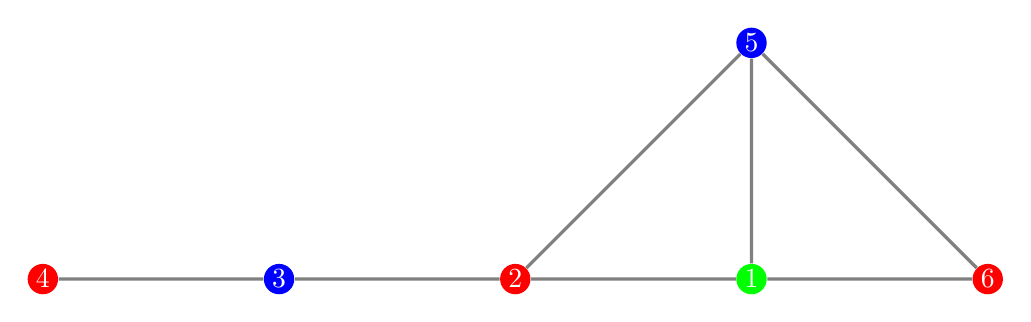
\begin{tikzpicture}[
        blue/.style={font=\color{white}\sffamily,fill=blue,circle,inner sep=1pt,minimum size=0.25cm},
        red/.style={font=\color{white}\sffamily,fill=red,circle,inner sep=1pt,minimum size=0.25cm},
        green/.style={font=\color{white}\sffamily,fill=green,circle,inner sep=1pt,minimum size=0.25cm},
        scale=3
    ]
    \node[red] (2) at (0,0) {$2$};
    \node[red] (4) at (-2,0) {$4$};
    \node[blue] (3) at (-1,0) {$3$};
    \node[green] (1) at (1,0) {$1$};
    \node[blue] (5) at (1,1) {$5$};
    \node[red] (6) at (2,0) {$6$};
    \draw[gray,very thick] (4)--(3) (3)--(2) (2)--(1) (1)--(6) (1)--(5) (5)--(2) (5)--(6); 
\end{tikzpicture}
\end{homeworkProblem}

\begin{homeworkProblem}
    The double of a graph G consists of two copies of G with edges joining corresponding vertices.
For example, a graph appears below on the left and its double appears on the right. Some
edges in the graph on the right are dashed to clarify its structure.

\includegraphics[scale=0.5]{./p3.png}
(a) Draw the double of the graph shown below.

\includegraphics[scale=0.5]{./p(a).png}
\newline
\newline
\solution

(a)

\includegraphics[scale=0.5]{./s4.png}

(b) Suppose that $G_1$ is a bipartite graph, $G_2$ is the double of $G_1,G_3$ is the double of $G_2$, and
so forth. Use induction on $n$ to prove that $G_n$ is bipartite for all $n \ge 1$.
\newline\newline
\solution

Base case is obvious , since we have $G_1$ is bipartite by definition.
\newline

Assume that $G_n$ is bipartite. We will construct 2-coloring for $G_{n + 1}$.
First off we are able to construct a 2-coloring for the two subgraphs($G'_{n}$ and $G''_{n}$) of $G_{n+1}$ which are isomorphic to $G_{n}$, for the fact that
$G_n$ is bipartite.
\newline

Now we examine the edges that connect $G'_{n}$ and $G''_{n}$. Let $v\in G'_{n}$, then $\forall w\in N_{v}$ we have $w\in G'_{n}$ xor $w\in G''_{n}$.
If $w\in G'_{n}$, and color$(v)$ is black, then by the bipartite graph property, color$(w)$ is white. If $w\in G''_{n}$, we set color$(w)$ = white.
We do the opposite operation of color$(v)$ is black. We then claim that $G''_{n}$ is then constructed with 2-color.
\newline

Assume the contrary that there are two vertices $x'', y''$ in $G''_{n}$ such that $x'', y''$ are of the same color and $\{x'', y''\}\in E$. By definition of the color construction, we have
the corresponding vertices $x', y'\in G'_{n}$ are also the same color but different from $\{x'', y''\}$. Then the path from $x''$ to $y''$ has even length.
but that is impossible since $x''$ to $y''$ has odd length.
\newline

Thus $G_{n+1}$ must be bipartite as well. By induction principle, $\forall n\in \N. G_{n}$ is bipartite.
\qed

\end{homeworkProblem}

\newpage

\begin{homeworkProblem}
Let $m, n$, and r be nonnegative integers with $r \le m$ and $r \le n$. Prove the following formula
by a combinatorial proof.
\[\binom{m + n}{r} = \sum_{k=0}^{r}\binom{m}{k}\binom{n}{r-k}\tag{*}\]

\solution

Let $S = \{1,\cdots, m + n\}$, $A = \{1,\cdots, n\}$, $B = \{n + 1, \cdots, m\}$.
We immediately have $S = A\cup B$, and $A\cap B = \{\}$.
\newline

On the one hand, $S$ has \[\binom{m + n}{r}\] subsets with cardinality $r$.
On the other hand, let $U_k \subseteq S$, with $|U_k| = r$. Then $U_k = S \cup T$, where $S\subseteq A$, and
$T\subseteq B$, Thus there are \[\binom{m}{k}\binom{n}{r-k}\]
such $U_k$ if $|S| = k$. Therefore the number of subsets of $S$ with cardinality $r$ can also
be expressed as 
    \[\sum_{k=0}^{r}|U_k| = \sum_{k=0}^{r}\binom{m}{k}\binom{n}{r-k}\]
Thus (*) has been proven.

\qed
\end{homeworkProblem}
\newpage
\begin{homeworkProblem}
    Establish the identity below using a combinatorial proof.
    \[\binom{2}{2}\binom{n}{2} + \binom{3}{2}\binom{n-1}{2}+\cdots+\binom{n}{2}\binom{2}{2} = \binom{n+3}{5}\]
\solution
\newline

We rewrite the identity as
    \[\sum_{k=0}^{n-1}\binom{k+2}{2}\binom{n-k}{2} = \binom{n+3}{5}\]
Consider $S = \{1,\cdots,n + 3\}$. Let $T_i\subseteq S$, with $|T_i| = 5$.
$T_i$ has pattern $T_i = A_{i}\cup \{i\}\cup B_{i}$, where $A_{i} \subseteq \{1,\cdots, i  -1 \}$, and $B_i\subseteq \{i + 1,\cdots, n + 3\}$,
with $|A_i| = |B_i| = 2$, and $i \in \{3,\cdots, n+1\}$
Thus, we have set $k = i - 2$

\begin{align*}
    \binom{n+3}{5} &= \left|\{T| T\subseteq S , |T| = 5\}\right| \\
                   &= \sum_{i=2}^{n+1}|T_i| \\
                   &= \sum_{i=2}^{n+1}\binom{i - 1}{2}\cdot 1 \cdot \binom{(n + 3) - (i - 1) - 1}{2}\\
                   &= \sum_{i=2}^{n+1}\binom{i - 1}{2}\binom{n+3-i}{2} \\
                   &= \sum_{k=0}^{n-1}\binom{k+2}{2}\binom{n-k}{2}
\end{align*}
\qed
\end{homeworkProblem}

\begin{homeworkProblem}
    Find the number of solutions of the equation $x_1 + x_2 + x_3 = 11$, where $x_1, x_2, x_3$ are nonnegative
integers with $x_1 \le 3, x_2 \le 4, x_3 \le 6$.
\newline

\solution
\newline

The generating function for this problem is

\newpage

\begin{align*}
    G(x) &= \left(1 + x + x^2 + x^3\right)\left(1+x+x^2+x^3+x^4\right)\left(1+x+x^2+x^3+x^4+x^5+x^6\right)\\
         &= \left(\frac{1}{1-x} - \frac{x^4}{1-x}\right)\left(\frac{1}{1-x} - \frac{x^5}{1-x}\right)\left(\frac{1}{1-x}-\frac{x^7}{1-x}\right)\\
         &= \frac{(1-x^4)(1-x^5)(1-x^7)}{(1-x)^3}\\
         &= (1-x^4)(1-x^5)(1-x^7)\sum_{k\ge 0}\binom{2+k}{k}x^k \\
         &= (1 + x^9 + x^{12} + x^{11} - x^{16} - x^4 - x^5 - x^7)\sum_{k\ge 0}\binom{2+k}{k}x^k
\end{align*}
Thus, the coefficient of $x^{11}$ in this function is
\[\binom{2+11}{11} + \binom{2 + 2}{2} + \binom{2+0}{0} - \binom{2 + 7}{7} - \binom{2+6}{6} - \binom{2+4}{4} = 6 \]

\qed
\end{homeworkProblem}

\begin{homeworkProblem}
    Show that in any set of $n + 1$ positive integers not exceeding $2n$ there must be two that are
relatively prime.
\newline

\solution
\newline

Let $S$ be a set of positive integers of $n + 1$ elements with the maximum element $m \le 2n$.
Let $m$ be the minimum element of $S$.
We claim that there are two elements in $S$, such that they differ by one.
\newline
Assume the contrary, there are no such elements. Then the maximum element of $S$ is at least
\[M \ge m + \sum_{k=1}^{n}2 = m + 2n\ge 1 + 2n > 2n\]
We have a contradiction then.

\qed 
\end{homeworkProblem}

\newpage

\begin{homeworkProblem}
A 0-1 sequence an with $2m$ terms is said to be normal if the following two conditions are
satisfied.
\begin{itemize}
    \item There exist $m$ terms equal to 0 and the other $m$ terms equal to 1 in an.
    \item For arbitrary $k \le 2m$, the number of terms equal to $0$ is not less than that of terms
    equal to $1$ in the first $k$ terms $a_1, a_2, \cdots , a_k$.
\end{itemize}

Please complete the following questions.
\newline 

(a) Show that the number of abnormal 0-1 sequences an with $2m$ terms equals that of sequences
an of which $(m + 1)$ terms are 0s and $(m - 1)$ terms are 1s.
\newline

(b) For $m = 4$, determine the number of different normal 0-1 sequences an. Note: An abnormal
0-1 sequence an is a 0-1 sequence that does not satisfy the properties of normal 0-1
sequences.
\newline

\solution
\newline

(a) Let $f:\{0, 1\} \to \{-1, 1\}$ be a function such that:

\begin{equation}
    f(n) =
    \begin{cases*}
      1 & if $n = 1$ \\
      -1        & if $n = 0$
    \end{cases*}
\end{equation}

The condition 2 for a normal sequence become
\[\forall n\in \{1, \cdots, 2m\} \sum_{k = 1}^{n}f(a_k) \ge 0\]
We consider a arbitrary sequence $\{b_1,\cdots, b_n\}$ with $m+1$ 1s, and $m-1$ zeros.
Let $A$ be the set of all abnormal sequences, and let $B$ be the set of all $(m+1)$ 1s sequences
We will construct a bijection from $A$ to $B$ 
We have
\[\sum_{k=0}^{2m}f(b_k) = 2\]
Thus there must be an minimal $m_0$ such that
\[\sum_{k=0}^{m_0}f(b_k) = 1\]
And deduced that
\[\sum_{k=m_0+1}^{2m}f(b_k) = 1\]
We construct $\sigma$ given by
\begin{equation}
    b_n \mapsto
    \begin{cases*}
      \mathrm{flip}(b_n) & for $n \le m_0$ \\
      b_n        & otherwise
    \end{cases*}
\end{equation}
where $\mathrm{flip}(0) = 1, \mathrm{flip}(1) = 0$
In this case we have 
\[\sum_{k=0}^{2m} f(\sigma(b_n)) = \sum_{k \le m_0}-f(b_n) + \sum_{k > m_0}f(b_n) = -1 + 1 = 0\]
Hence $\sigma(b_n)$ is a abnormal sequence. Note that it is easy to check that the $\mathrm{flip}$ function is 1-1, then so is 
$\sigma$. We now need to show that $\sigma$ is also on-to. Let $\{a'_n\}$ be an abnormal sequence, by its definition
there is a minimal $n_0$ such that 
\[\sum_{k=0}^{n_0}f(a'_k) = -1\]

We choose a sequence $\{b'_n\}_{1}^{2m} = \{\flip(a'_1),\cdots,\flip(a'_{n_0}),\cdots, a'_{n_0 + 1},\cdots, a'_{2m}\}$
We compute
\[\sum_{b\in \{b'_n\}_{1}^{2m}} f(b) = \sum_{k = 0}^{n_0}\flip(a'_{k})  + \sum_{k > n_0} f(a'_{k}) = 1 + 1 = 2\]
Thus $\{b'_n\}_{1}^{2m} \in B$, and we have the bijection constructed.
\qed
\newline

(b) The number of normal sequence is obtained by the number of sequences minus the number of abnormal sequences, that is .
\[\binom{2n}{n} - \binom{2n}{n + 1}\]

Thus the answer to this question is 
\[\binom{2\times 4}{4} - \binom{2 \times 4}{4 + 1} = 70-56 = 14\]

\qed

\end{homeworkProblem}

\end{document}